\documentclass[notitlepage]{article}

\usepackage{amsmath}
\let\vec\mathbf
\usepackage{graphicx}
\usepackage{caption}
\usepackage{rotating}
\usepackage{float}
\usepackage[margin=0.8in]{geometry}
\usepackage[section]{placeins}
\usepackage[hidelinks]{hyperref}
\usepackage{bytefield}
\usepackage{siunitx}
\usepackage{csquotes}
\MakeOuterQuote{"}

\newcommand{\reservedfield}{\color{lightgray}\rule{\width}{\height}}

\setlength{\parskip}{0.3em}
\usepackage{xcolor}
\usepackage{listings}
\lstset{
	language=Verilog,
	frame=single,
	basicstyle=\small,
	keywordstyle=\color{blue}\small,
	stringstyle=\color{Maroon}\small,
	commentstyle=\color{OliveGreen}\small,
	breaklines=true,
	postbreak=\raisebox{0ex}[0ex][0ex]{\ensuremath{\color{red}\hookrightarrow\space}}
}

\title{RISCBoy Documentation}
\author{Luke Wren}
\date{}
\makeatletter
\newcommand*{\toccontents}{\@starttoc{toc}}
\makeatother

\begin{document}

\pagenumbering{gobble}
\maketitle
\toccontents
\listoffigures
\newpage
\pagenumbering{arabic}

\include{ch1_intro}
\include{ch2_cpu_architecture}
\section{Pixel Processing Unit (PPU)}

Figure \ref{diagram:ppu_block} shows the high-level structure of the PPU. This is the second-generation architecture -- the previous version had a number of sprite and tile engines operating in parallel, with shared bus access. This was a mistake. Many of these units were idle much of the time, and they were stripped down to the minimum to meet strict area requirements; this in turn led to poor bus utilisation and a lack of flexibility. The second problem was partially solved by the Poker, but at the expense of high software complexity for common use cases (e.g. many sprites on screen). The high level goals of PPU2 are, in order of precedence:

\begin{enumerate}
\item Always Be Fetching
\item Avoid idle or duplicated base functional units (e.g. pixel unpacker) so that more expensive functions can be provided (e.g. random access to pixels)
\item Be highly programmable, and allow features to be combined in interesting ways
\item Serve the simple use cases (layered, tiled backgrounds with sprites) with minimum program complexity
\item Mario Kart: Super Circuit
\end{enumerate}

Fundamentally we are fetching pixels from memory (over a 16 bit bus on RISCBoy), and putting them on the screen in interesting orders. If we saturate the bus, and do not waste what we fetch, our performance is as good as it possibly can be.

\begin{figure}[H]
\centering
\caption{Pixel processing unit, block-level diagram}
\label{diagram:ppu_block}
\includegraphics[width=\textwidth]{diagrams/ppu_block.pdf}
\end{figure}

At any point in time the PPU is either rendering to one of the internal scanline buffers, or waiting for a buffer to be freed and passed back by the display interface hardware. The exact sequence of operations the PPU performs while rendering is defined by a program in memory, executed by the command processor. The instruction set is small, and specialised to the task at hand -- for example the {\tt SYNC} instruction marks the current scanline buffer as ready for display, and waits for a buffer be freed by the display hardware, and the {\tt FILL} instruction writes a constant-colour span to some $x$ range of pixels.

Common memory access patterns (for nonpaletted pixels):

\begin{itemize}
	\item Sprite blitting: fetch a pixel from memory every cycle
	\item Tiling: fetch a tile index after every $n$ pixels, then $n$ pixel fetches
	\item Affine-mapped tiling: fetch tile indices and pixels on alternate cycles
\end{itemize}

The display controller attaches to a dedicated interface on the PPU. Through a simple handshake, the display controller can acquire and release dirty scanbuffers. The display interface routes read addresses from the display controller to the correct scanline buffer, and routes pixel data back to the controller. Currently two display controllers are available to connect to this interface: one for serial LCDs such as ILI9341, and another for direct DVI output. The PPU display interface is synchronous, and any clock crossing (to SCK domain for serial LCDs, or pixel clock domain for DVI) is handled inside the display controller.

\subsection{Pixel Formats}

Internally, the PPU uses a single native pixel format, namely ARGB 1555 (see figure \ref{diagram:pixformat}), but it can stream pixels from memory in a variety of formats, and convert internally. PPU memory accesses are \textbf{always little-endian}: for performance reasons the PPU performs the widest possible fetch, yielding multiple pixels each, which are numbered least-significant-first.

\begin{figure}[H]
\centering
\caption{PPU pixel formats}
\label{diagram:pixformat}
\begin{tabular}{r l}
	\raisebox{-1ex}[5ex][1.5ex]{
		\begin{bytefield}[endianness=big,bitformatting=\small, bitwidth=auto]{16}
		\bitheader{0,4,5,9,10,14,15} \\
		\bitbox{1}{A} \bitbox{5}{R} \bitbox{5}{G} \bitbox{5}{B}
		\end{bytefield}} & Mode 0: ARGB1555, alpha = 0 when transparent \\
		\\
	\raisebox{-1ex}[5ex][1.5ex]{
		\begin{bytefield}[endianness=big,bitformatting=\small, bitwidth=auto]{8}
		\bitheader{0,7} \\
		\bitbox{8}{Index}
		\end{bytefield}} & Mode 1: P8, an index into a table of 256 colours\\
		\\
	\raisebox{-1ex}[5ex][1.5ex]{
		\begin{bytefield}[endianness=big,bitformatting=\small, bitwidth=auto]{4}
		\bitheader{0,3} \\
		\bitbox{4}{Index}
		\end{bytefield}} & Mode 2: P4, an index into a table of 16 colours \\
		\\
	\raisebox{-1ex}[5ex][1.5ex]{
		\begin{bytefield}[endianness=big,bitformatting=\small, bitwidth=auto]{1}
		\bitheader{0} \\
		\bitbox{1}{I}
		\end{bytefield}} & Mode 3: P1, an index into a table of 2 colours \\
		\\
\end{tabular}
\end{figure}

For pixels smaller than one byte, the pixel order continues to be defined in a little-endian fashion, i.e. the least-significant pixel will be the first to be displayed. The PPU also requires image base addresses to be word-aligned, which implies all pixels are naturally aligned.

\subsection{Palettes}

The PPU contains a single hardware palette memory (PRAM), which is large enough to store 256 colours in ARGB1555 format. Each pixel in a paletted image (see figure \ref{diagram:pixformat}) consists of an index into PRAM. The PPU looks these indices up before passing pixels to the screen; wide colour range is maintained at reduced bits per pixel.

Since PRAM contents is in ARGB1555 format, there is no special convention for indicating whether a paletted pixel is transparent: the hardware always performs the palette lookup, and the resulting colour may or may not have its Alpha bit set.

Although there is only a single hardware palette, 256 colours in size, {\tt TILE} and {\tt BLIT} commands can supply an offset, which is added to each paletted pixel before palette lookup. PRAM may be initialised with e.g. multiple 16-colour tables at different (potentially overlapping) locations, giving effectively independent palettes.

PRAM can be written to (but not read) through the PPU's configuration interface.

\subsection{Scanline Buffers}


The scanline buffers are implemented as 1-read 1-write memories, which allows the blending pipeline to easily achieve a 1 pixel per clock throughput, keeping the bottleneck on the system bus. This could also be implemented as a double-width 1RW memory, but not a compelling tradeoff on FPGA.

\begin{figure}[H]
\centering
\caption{PPU scanline buffer states}
\label{diagram:ppu_buffer_states}
\includegraphics[width=0.7\textwidth]{diagrams/ppu_buffer_states.pdf}
\end{figure}

On RISCBoy these are 15b$\times512$ memories, each composed of a pair of iCE40 4~kb block RAMs. This is sufficient to store one QVGA RGB555 scanline in each buffer. The blitter and display pass each other buffers through a pair of queues, one containing clean buffers for the blitter, and the other containing dirty buffers for the display. After reset, both buffers are in the clean queue.

\subsection{Instruction Set}

Each instruction consists of one or more words in memory; the blitter processes each instruction in turn, progressing in a linear fashion unless a {\tt POPJ} is encountered, or the PPU is manually vectored to a new program by system software. This section describes the encoding of blitter instructions, and their operation. Some fields are marked as {\it reserved}, denoted by a grey colour fill in the bit diagrams. Reserved fields are not used by the current hardware, and should be written all-zeroes by software.

For simple purposes (e.g. tiled backgrounds with some sprites on top), the blitter can execute the same program on each scanline: the coordinate systems of {\tt BLIT}/{\tt TILE} commands take the current raster $y$ coordinate into account (see section \ref{section:coordinates}). However, the instruction set is quite flexible, and the blitter's features can be combined in interesting ways, with fancy-looking results.

\subsubsection*{SYNC}

\begin{bytefield}[endianness=big,bitformatting=\tiny]{32}
\bitheader{0,27,28,31} \\
\bitbox{4}{{\tt 0x0}} \bitbox{28}{\reservedfield} \\
\end{bytefield}

Present the current scanline buffer to the display, then stall until a clean buffer becomes available. If {\tt CSR\_HALT\_HSYNC} is set, or {\tt CSR\_HALT\_VSYNC} is set and this is the last line of the frame, halt the PPU.

\subsubsection*{CLIP}

\begin{bytefield}[endianness=big,bitformatting=\tiny]{32}
\bitheader{0,9,10,19,20,27,28,31} \\
\bitbox{4}{{\tt 0x1}} \bitbox{8}{\reservedfield} \bitbox{10}{{\tt x\_end}} \bitbox{10}{{\tt x\_start}} \\
\end{bytefield}

Set the active region for rendering. Pixels at $x$ coordinates less than {\tt x\_start} or greater than {\tt x\_end} will be unaffected by subsequent {\tt FILL}, {\tt [A]TILE} or {\tt [A]BLIT} operations. This region remains in effect until another {\tt CLIP} is executed.

Often it is sufficient to perform an initial {\tt CLIP} to the screen width, and never change from this value, but {\tt CLIP} has numerous applications when combined with pixel-filling operations: for example using {\tt CLIP} + {\tt ABLIT} pairs to render a sequence of short affine-textured spans.

\subsubsection*{FILL}

\begin{bytefield}[endianness=big,bitformatting=\tiny]{32}
\bitheader{0,4,5,9,10,14,15,27,28,31} \\
\bitbox{4}{{\tt 0x2}} \bitbox{13}{\reservedfield} \bitbox{5}{{\tt R}} \bitbox{5}{{\tt G}} \bitbox{5}{{\tt B}} \\
\end{bytefield}

Fill the entire clipped region with a single colour. Note that scanline buffers retain their old contents when passed back to the blitter by the display hardware; if you want a solid background colour, you must {\tt FILL} it into each scanline, or include it in your background tileset.

\subsubsection*{BLIT}

\begin{bytefield}[endianness=big,bitformatting=\tiny]{32}
\bitheader{0,9,10,19,20,21,22,24,25,27,28,31} \\
\bitbox{4}{{\tt 0x4}} \bitbox{3}{{\tt size}} \bitbox{3}{{\tt poff}} \bitbox{2}{\reservedfield} \bitbox{10}{{\tt y}} \bitbox{10}{{\tt x}} \\
\bitheader{0,1,2, 31} \\
\bitbox{30}{{\tt img}} \bitbox{2}{\tt fmt} \\
\end{bytefield}

Block image transfer: paste a square image (e.g. a sprite) over the current scanline. If this image does not intersect the current scanline due to its position and size, or if it is fully outside of the clipped region on this scanline, the {\tt BLIT} command has no effect, and completes immediately. Generally {\tt BLIT} is called on each scanline with the same arguments, to build up the full image. For example, each game sprite may correspond to a {\tt BLIT} command which runs on every scanline.

{\tt BLIT} also supports efficient framebuffer graphics: in this case each scanline will have a different {\tt BLIT} command with a {\tt y} equal to that scanline's position, and a {\tt img} pointer that is one scanline further advanced into a software framebuffer. This allows a framebuffer to be packed in memory as a flat $\textup{width} \times \textup{height}$ array of pixels.

\begin{itemize}
\item {\tt img} is a pointer to the source image, which is assumed to be word-aligned (hence the missing LSBs).
\item {\tt fmt} is the pixel format, as described in figure \ref{diagram:pixformat}. The values are: mode 0 ARGB1555, mode 1 P8, mode 2 P4, mode 3 P1.
\item {\tt size} defines the size of the source image: $\textup{width}=\textup{height}=2^{{\tt size} + 3}$, so square images from 8 to 1024 pixels are supported.
\item {\tt poff} is the palette offset. This is left-shifted by 5 and added to each paletted pixel, with wrap on overflow, before the pixel is looked up in the palette RAM.
\end{itemize}

\subsubsection*{TILE}

\begin{bytefield}[endianness=big,bitformatting=\tiny]{32}
\bitheader{0,9,10,19,20,21,22,24,25,26,27,28,31} \\
\bitbox{4}{{\tt 0x5}} \bitbox{2}{\reservedfield} \bitbox{1}{{\tt s}} \bitbox{3}{{\tt poff}} \bitbox{2}{\reservedfield} \bitbox{10}{{\tt yscroll}} \bitbox{10}{{\tt xscroll}} \\
\bitheader{0,1,2, 31} \\
\bitbox{30}{{\tt tilemap}} \bitbox{2}{{\tt pfs}} \\
\bitheader{0,1,2, 31} \\
\bitbox{30}{{\tt tileset}} \bitbox{2}{\tt fmt} \\
\end{bytefield}

Render a tiled background span (see section \ref{section:tiles}).

\begin{itemize}

\item {\tt xscroll} and {\tt yscroll} define the horizontal and vertical scroll of the tiled region. (TBD this may need to be redefined slightly for new PPU).

\item {\tt s} defines the size of the source image: $\textup{width}=\textup{height}=2^{{\tt s} + 3}$, so square images of $8\times 8$ or $16\times 16$ are supported.

\item {\tt poff} is the palette offset. This is left-shifted by 5 and added to each paletted pixel, with wrap on overflow, before the pixel is looked up in the palette RAM.

\item {\tt tileset} is a pointer to an array of $8\times 8$ or $16\times 16$~px images

\item {\tt fmt} is the pixel format of the tileset images, as described in figure \ref{diagram:pixformat}. The values are: mode 0 ARGB1555, mode 1 P8, mode 2 P4, mode 3 P1.

\item {\tt tilemap} is a pointer to a 2D array of 8 bit tile indices. Each index identifies which image from {\tt tileset} occupies that $8\times 8$ or $16\times 16$~px square.

\item {\tt pfs} is the playfield size in pixels, $\textup{width}=\textup{height}=2^{{\tt size} + 7}$, so 128 to 1024 px. See section \ref{section:tiles}.
\end{itemize}

\subsubsection*{ABLIT}

\begin{bytefield}[endianness=big,bitformatting=\tiny]{32}
\bitheader{0,9,10,19,20,21,22,24,25,27,28,31} \\
\bitbox{4}{{\tt 0x6}} \bitbox{3}{{\tt size}} \bitbox{3}{{\tt poff}} \bitbox{1}{\tt h} \bitbox{1}{\reservedfield} \bitbox{10}{{\tt y}} \bitbox{10}{{\tt x}} \\
\bitheader{0,15,16, 31} \\
\bitbox{16}{\tt b1} \bitbox{16}{\tt b0} \\
\bitheader{0,15,16, 31} \\
\bitbox{16}{\tt a01} \bitbox{16}{\tt a00} \\
\bitheader{0,15,16, 31} \\
\bitbox{16}{\tt a11} \bitbox{16}{\tt a10} \\
\bitheader{0,1,2, 31} \\
\bitbox{30}{{\tt img}} \bitbox{2}{\tt fmt} \\
\end{bytefield}


Like {\tt BLIT}, except screen coordinates are transformed before each pixel lookup:

\begin{align*}
\vec{u}   &= \vec{A}(\vec{s} - \vec{s}_0) + \vec{b} \\
\end{align*}

Where

\begin{align*}
\vec{u}   &= \begin{bmatrix}u & v \\ \end{bmatrix}^T & \textup{(texture coordinates)} \\
\vec{s}   &= \begin{bmatrix}s_x & s_y \\ \end{bmatrix}^T & \textup{(screen coordinates)} \\
\vec{s}_0 &= \begin{bmatrix}x & y \\ \end{bmatrix}^T & \textup{(blit target position {\tt x}, {\tt y})} \\
\vec{A}   &= \begin{bmatrix}a_{00} & a_{01} \\ a_{10} & a_{11} \end{bmatrix} & \textup{(scale/rotate/shear matrix)} \\
\vec{b}   &= \begin{bmatrix}b_0 & b_1 \\ \end{bmatrix}^T & \textup{(translation vector)} \\
\end{align*}

This affine transform is described in detail in section \ref{section:affine_transform}. It allows a range of geometric manipulations of the source image. {\tt ABLIT} renders to the same square region as {\tt BLIT}, defined by the {\tt size}, {\tt x} and {\tt y} parameters, as well as the current {\tt CLIP} region. It is the {\it texture lookup} for each rendered pixel that differs.

The {\tt a} components are signed 8.8 fixed point numbers, and {\tt b} components are unsigned 10.6 fixed point.
\begin{itemize}
	\item {\tt h}: half-size flag: indicate the texture is only half the size of the rasterized region in each axis. This allows e.g. a $32\times 32$~px texture to be rotated, without scaling, by \ang{45} and blitted to a $64\times64$~px region, so that its corners are not clipped. The effect of the half-size flag when {\tt size} = 0 is undefined.
	\item {\tt img} is a pointer to the source image, which is assumed to be word-aligned (hence the missing LSBs).
	\item {\tt fmt} is the pixel format, as described in figure \ref{diagram:pixformat}. The values are: mode 0 ARGB1555, mode 1 P8, mode 2 P4, mode 3 P1.
	\item {\tt size} defines the size of both the source image and the blit target area: $\textup{width}=\textup{height}=2^{{\tt size} + 3}$, so square images from 8 to 1024 pixels are supported.
	\item {\tt poff} is the palette offset. This is left-shifted by 5 and added to each paletted pixel, with wrap on overflow, before the pixel is looked up in the palette RAM.
\end{itemize}

\subsubsection*{ATILE}

\begin{bytefield}[endianness=big,bitformatting=\tiny]{32}
\bitheader{0,9,10,19,20,21,22,24,25,26,27,28,31} \\
\bitbox{4}{{\tt 0x7}} \bitbox{2}{\reservedfield} \bitbox{1}{{\tt s}} \bitbox{3}{{\tt poff}} \bitbox{2}{\reservedfield} \bitbox{10}{{\tt yscroll}} \bitbox{10}{{\tt xscroll}} \\
\bitheader{0,15,16, 31} \\
\bitbox{16}{\tt b1} \bitbox{16}{\tt b0} \\
\bitheader{0,15,16, 31} \\
\bitbox{16}{\tt a01} \bitbox{16}{\tt a00} \\
\bitheader{0,15,16, 31} \\
\bitbox{16}{\tt a11} \bitbox{16}{\tt a10} \\
\bitheader{0,1,2, 31} \\
\bitbox{30}{{\tt tilemap}} \bitbox{2}{{\tt pfs}} \\
\bitheader{0,1,2, 31} \\
\bitbox{30}{{\tt tileset}} \bitbox{2}{\tt fmt} \\
\end{bytefield}

Like {\tt TILE} but affine transform applied before each tile and pixel lookup: $\vec{u} = \vec{A}(\vec{s} - \vec{s}_0) + \vec{b}$. As with {\tt TILE}, the entire {\tt CLIP} region is rendered to. $\vec{s}_0$ is the {\tt xscroll}, {\tt yscroll} offset, the same as {\tt TILE}. All in all, {\tt TILE} can be thought of as a simple case of {\tt ATILE}, where $\vec{A}$ is the identity matrix and $\vec{b}$ is the zero vector.

\begin{itemize}
	\item {\tt s} defines the size of the source image: $\textup{width}=\textup{height}=2^{{\tt s} + 3}$, so square images of $8\times 8$ or $16\times 16$ are supported.
	\item {\tt poff} is the palette offset. This is left-shifted by 5 and added to each paletted pixel, with wrap on overflow, before the pixel is looked up in the palette RAM.
	\item {\tt tileset} is a pointer to an array of $8\times 8$ or $16\times 16$~px images
	\item {\tt fmt} is the pixel format of the tileset images, as described in figure \ref{diagram:pixformat}. The values are: mode 0 ARGB1555, mode 1 P8, mode 2 P4, mode 3 P1.
	\item {\tt tilemap} is a pointer to a 2D array of 8 bit tile indices. Each index identifies which image from {\tt tileset} occupies that $8\times 8$ or $16\times 16$~px square.
	\item {\tt pfs} is the playfield size in pixels, $\textup{width}=\textup{height}=2^{{\tt size} + 7}$, so 128 to 1024 px. See section \ref{section:tiles}.
\end{itemize}

\subsubsection*{PUSH}

\begin{bytefield}[endianness=big,bitformatting=\tiny]{32}
\bitheader{0,27,28,31} \\
\bitbox{4}{{\tt 0xe}} \bitbox{28}{\reservedfield} \\
\bitheader{0, 1, 2, 31} \\
\bitbox{30}{\tt data} \bitbox{2}{\reservedfield} \\
\end{bytefield}

Push literal {\tt data} onto the stack. The stack is popped only by a {\tt POPJ} instruction, is 8 words deep, and wraps on empty/full.

\subsubsection*{POPJ}

\begin{bytefield}[endianness=big,bitformatting=\tiny]{32}
\bitheader{0,9,10,23,24,27,28,31} \\
\bitbox{4}{{\tt 0xf}} \bitbox{4}{\tt cc}  \bitbox{14}{\reservedfield} \bitbox{10}{{\tt a}} \\
\end{bytefield}

Always pop an address from the stack. If {\tt cc} is true, branch to this address. Values for {\tt cc}:

\begin{itemize}
	\item 0: always
	\item 1: YLT, current raster beam $y < {\tt a}$
	\item 2: YGE, current raster beam $y \geq {\tt a}$
\end{itemize}

A regular jump is formed with {\tt PUSH addr; POPJ}, and a subroutine call is formed with {\tt PUSH ret; PUSH target; POPJ; label ret:} followed by a {\tt POPJ} at the end of the target routine.

Subroutines are useful for when a part of your command list is repeated every scanline (e.g. a list of sprites, represented by {\tt BLIT} commands) and a part is not (e.g. {\tt FILL}ing a different background colour every scanline to produce a gradient). Such a program can be structured as a larger per-frame command list which repeatedly calls into a per-scanline subroutine.


\subsection{Coordinate Systems}
\label{section:coordinates}

The origin of the screen is at the top left. $x$ coordinates increase to the right. $y$ coordinates increase going downward.


\begin{figure}[H]
\centering
\caption{PPU screen coordinate system}
\label{diagram:ppu_coord_screen}
\includegraphics[width=0.4\textwidth]{diagrams/ppu_coord_screen.pdf}
\end{figure}

When using a vector to refer to a screen-space coordinate, we will typically use the symbol $\vec{s}$.

\subsubsection*{Texture Coordinates}

\begin{figure}[H]
\centering
\caption{PPU texture coordinate system}
\label{diagram:ppu_coord_texture}
\includegraphics[width=0.25\textwidth]{diagrams/ppu_coord_texture.pdf}
\end{figure}

Textures (e.g. sprite images) have completely independent coordinates. We will conventionally refer to pixels in texture space with the vector $\vec{u} = \begin{bmatrix} u & v \\ \end{bmatrix}^T$. Textures are stored in memory as a flat array of pixels, going first in $u$ order and then stepping down to the next row.

When drawing a sprite, the PPU does the following:

\begin{itemize}
	\item Iterate over each pixel in some horizontal span of screen space
	\item For each pixel, transform the screen-space coordinate $\vec{s}$ into a texture-space coordinate $\vec{u}$
	\item Look up the texture pixel at $\vec{u}$ and draw it on the screen at $\vec{s}$
\end{itemize}

This transformation may be simple, as in the case of the {\tt BLIT} command:

\[
\vec{u} = \vec{s} - \vec{s}_0
\]

Where $\vec{s}_0$ is the position the texture is being blitted to ({\tt x}, {\tt y} in the {\tt BLIT} instruction), $\vec{s}$ is the position of next pixel to be rendered on the screen, and $\vec{u}$ is the position in texture space which determines the colour of the screen pixel. The transformation may be more complex, as in the case of the {\tt ABLIT} command:

\[
\vec{u} = \vec{A}(\vec{s} - \vec{s}_0) + \vec{b}
\]

Where the matrix $\vec{A}$ and vector $\vec{b}$ are constants supplied by the {\tt ABLIT} instruction, permitting any combination of translation, rotation, scale and shear. Note the direction of the definition: this is a mapping {\it from} screen space {\it to} texture space. If you find it more intuitive to think about mapping the texture onto the screen, you must note that this is the {\it inverse} of the above mapping, and you have some linear algebra to do.

Internally, the PPU represents $\vec{u}$-space coordinates as pairs of unsigned 10.8 fixed point numbers (a range of $0$ to $1023 + \frac{255}{256}$); the largest supported texture size is therefore $1024 \times 1024$~px.

As far as coordinates are concerned, there is no difference between e.g. a $512\times 512$~px texture and a $512\times 512$~px tiled background. The difference is that a texture's pixels are defined by a single large image ($512 \times 512$~px in this example), whereas the tiled area is defined by a number of small e.g. $16 \times 16$~px images called the {\it tileset}, and a 2D array of tile indices called the {\it tilemap} which defines which $16 \times 16$~px image should be at which $16 \times 16$~px region of $\vec{u}$-space.

\subsubsection*{Affine Transforms}
\label{section:affine_transform}

We gave the following definition for the transformation from screen space to texture space used by the {\tt ABLIT} and {\tt ATILE} commands:

\[
\vec{u} = \vec{A}(\vec{s} - \vec{s}_0) + \vec{b}
\]

All of our examples will use the following texture which, for argument's sake, is $64 \times 64$~px in size:

\begin{figure}[H]
\centering
\caption{PPU texture example}
\label{diagram:ppu_texture_example}
\includegraphics[width=0.25\textwidth]{diagrams/ppu_texture_example.pdf}
\end{figure}


Like {\tt BLIT}, {\tt ABLIT} renders to a square area of the screen, starting at $\vec{s}_0$ (defined by the {\tt x}, {\tt y} arguments to {\tt ABLIT}), and extending rightward and downward by the texture size.  If we set $\vec{A} = \vec{I} = \begin{bmatrix} 1 & 0 \\ 0 & 1 \\ \end{bmatrix}$ and $\vec{b} = \begin{bmatrix} 0 & 0 \\ \end{bmatrix}^T$, then the texture coordinate $\vec{u}$ is equal to the raster coordinate $\vec{s}-\vec{s}_0$, and the {\tt ABLIT} behaves the same as a {\tt BLIT}:

\begin{figure}[H]
\centering
\caption{PPU affine blit with identity mapping}
\label{diagram:ppu_texture_ablit01}
\includegraphics[width=0.8\textwidth]{diagrams/ppu_texture_ablit01.pdf}
\end{figure}

Setting $\vec{A}$ to the identity matrix maps the screen-space unit vectors $\vec{e}_x$ and $\vec{e}_y$ to the texture space's unit vectors $\vec{e}_u$, $\vec{e}_v$. The texture is undistorted. If we instead set $\vec{A} = \begin{bmatrix} 0 & 1 \\ 1 & 0 \\ \end{bmatrix}$:

\begin{figure}[H]
\centering
\caption{PPU affine blit with reflection in u=v}
\label{diagram:ppu_texture_ablit02}
\includegraphics[width=0.8\textwidth]{diagrams/ppu_texture_ablit02.pdf}
\end{figure}

The horizontal axis in screen space ($\vec{e}_x$) has instead been mapped to the vertical axis in texture space ($\vec{e}_v$), and vice versa. Texture lookups have been reflected across the line $u=v$.

We can perform a uniform scale by setting $\vec{A} = \lambda \vec{I}$, which maps the screen-space unit vectors onto {\it larger} vectors in texture space, so that texture samples of neighbouring screen pixels are further apart on the texture. E.g. take $\lambda=2$:

\begin{figure}[H]
\centering
\caption{PPU affine blit with uniform scale}
\label{diagram:ppu_texture_ablit03}
\includegraphics[width=0.8\textwidth]{diagrams/ppu_texture_ablit03.pdf}
\end{figure}

The $\vec{b}$ vector is used to translate texture lookups. It can be understood as the point in texture space to which the upper-left of the rasterised region is mapped, since at this point on the screen $\vec{s} = \vec{s}_0$, so $\vec{u} = \vec{A}(\vec{s}_0 - \vec{s}_0) + \vec{b} = \vec{b}$. For example, we could set $\vec{b} = \begin{bmatrix} -32 & -32 \\ \end{bmatrix}^T$, so that the sample corresponding to $\vec{s}_0$ is higher and further left in texture space:

\begin{figure}[H]
\centering
\caption{PPU affine blit with uniform scale and translation}
\label{diagram:ppu_texture_ablit04}
\includegraphics[width=0.8\textwidth]{diagrams/ppu_texture_ablit04.pdf}
\end{figure}

Figure \ref{diagram:ppu_texture_ablit04} shows $\vec{b}$ plotted in texture space, and the resulting shift of the sampled texture as seen in the rasterised area. For a final example, the matrix

\[
\vec{A} = \begin{bmatrix}
\cos\theta & -\sin\theta \\
\sin\theta & \cos\theta \\
\end{bmatrix}
\]

Defines, in our coordinate system, a clockwise rotation by $\theta$. Setting $\theta=45^{\circ}$, scaling by 2 and carefully choosing the $\vec{b}$ vector, we can make the texture appear to rotate {\it counterclockwise} about its centre in screen space.

\begin{figure}[H]
\centering
\caption{PPU affine blit with rotation}
\label{diagram:ppu_texture_ablit05}
\includegraphics[width=0.8\textwidth]{diagrams/ppu_texture_ablit05.pdf}
\end{figure}

Note that, without a scale factor, the corners of the texture would be clipped to the rasterised region of the screen. It is quite inefficient to take a large texture and always show it in a scaled-down form; {\tt ABLIT}'s half-size flag reduces the texture size to half of the rasterised region, so a $64\times 64$~px {\tt ABLIT} would expect a $32\times 32$~px texture, which would occupy the upper-left quadrant of the rasterised region if $\vec{A}=\vec{I}$ and $\vec{b}=\vec{0}$. This could then be rotated without scaling, and provided it is appropriately translated, the corners of the texture would not be clipped.

\subsection{Tiles}
\label{section:tiles}

To reduce memory footprint, the PPU is able to assemble scenes on the fly from an array of small images, known as tiles. TODO much of this section refers to old hw with dedicated tiled backgrounds engines

\begin{figure}[H]
\centering
\caption{PPU background coordinate system}
\label{diagram:ppu_bg_coords}
\includegraphics[width=0.7\textwidth]{diagrams/ppu_bg_coords.pdf}
\end{figure}

Each tile is a square image, the width and height of which (measured in pixels) is configured per-background, and is always a power of two. Tiles are stored as part of a larger image, known as the tileset. Tiles are numbered in a row-major order, starting at the top left of the tileset. An example tileset is shown in figure \ref{diagram:ppu_tileset}: this is a tileset of 8 tiles, each $4\times 4$ pixels in size.

\begin{figure}[H]
\centering
\caption{Example PPU tileset}
\label{diagram:ppu_tileset}
\includegraphics[width=0.7\textwidth]{diagrams/ppu_tileset.pdf}
\end{figure}

Each pixel row of the tileset is stored as a packed array of pixels in memory, and the next row follows. Note that all tiles must be the same size, and have the same pixel format.

The complete background image is assembled from these tiles. The arrangement is specified the tilemap: a grid of numbers, each naming a tile from the tileset. For each pixel on the screen, the tilemap tells the PPU which tile should be at that location, and the corresponding tile image in the tileset tells the PPU the colour of each pixel in that screen tile. This is shown in figure \ref{diagram:ppu_tilemap}.

\begin{figure}[H]
\centering
\caption{Example PPU tilemap}
\label{diagram:ppu_tilemap}
\includegraphics[width=0.7\textwidth]{diagrams/ppu_tilemap.pdf}
\end{figure}

The screen origin is offset into the background by configuring the horizontal and vertical scroll. This allows the game view to move smoothly over a fixed background. If the screen area overhangs the background, coordinates are wrapped.

In total, a background is defined by:

\begin{itemize}
	\item Width and height, measured in pixels
	\item Horizontal and vertical scroll, measured in pixels
	\item Tileset:
	\begin{itemize}
		\item Tile pixel format
		\item Tile size in pixels (power of two)
		\item Tileset width in pixels (power of two)
		\item Pointer to the tileset image (aligned to row size in bytes)
	\end{itemize}
	\item Tilemap:
	\begin{itemize}
		\item Pointer to the tilemap buffer
	\end{itemize}
\end{itemize}

This tilemapping process allows detailed images to be displayed with a minimal memory footprint, compared with a framebuffer, which must store the colour of every single pixel on the screen.

\section{Audio Processing Unit (APU)}

{\it Note: this section is even less complete than the others}

The APU is a lightweight processing core, designed to synthesise polyphonic audio, stream PCM or ADPCM audio from the system, or a mixture of the two, whilst blending/panning the audio channels. It runs in hard real time: each audio sample is calculated in one sample period, so no data buffering is required between APU and DACs. The design goals are:

\begin{enumerate}
	\item Low resource utilisation ($~100$ LUTs for the processing core)
	\item Output 48 kSa/s 8-bit stereo audio with a 12 MHz clock
	\item Provide similar interface to an 8-bit era games console with default APU code, so no programming required
	\item Streaming PCM audio from the system should be trivial (ring buffer + IRQ)
	\item Be fun to program: very focused on a single task, so quirky but easy to learn
\end{enumerate}

\subsection*{Architectural Overview}

\subsubsection*{Memory Architecture}

The APU is designed around a pair of iCE40 block RAMs: each is 16 bits wide by 256 entries deep, and has an independent read port and write port. The architecture and microarchitecture are designed around these parameters, for efficient use of the memory, and in particular for high utilisation of the memory ports. Figure \ref{diagram:apu_mem_arch} shows this in overview.

\begin{figure}[H]
\centering
\caption{Audio processing unit memory architecture}
\label{diagram:ppu_arch}
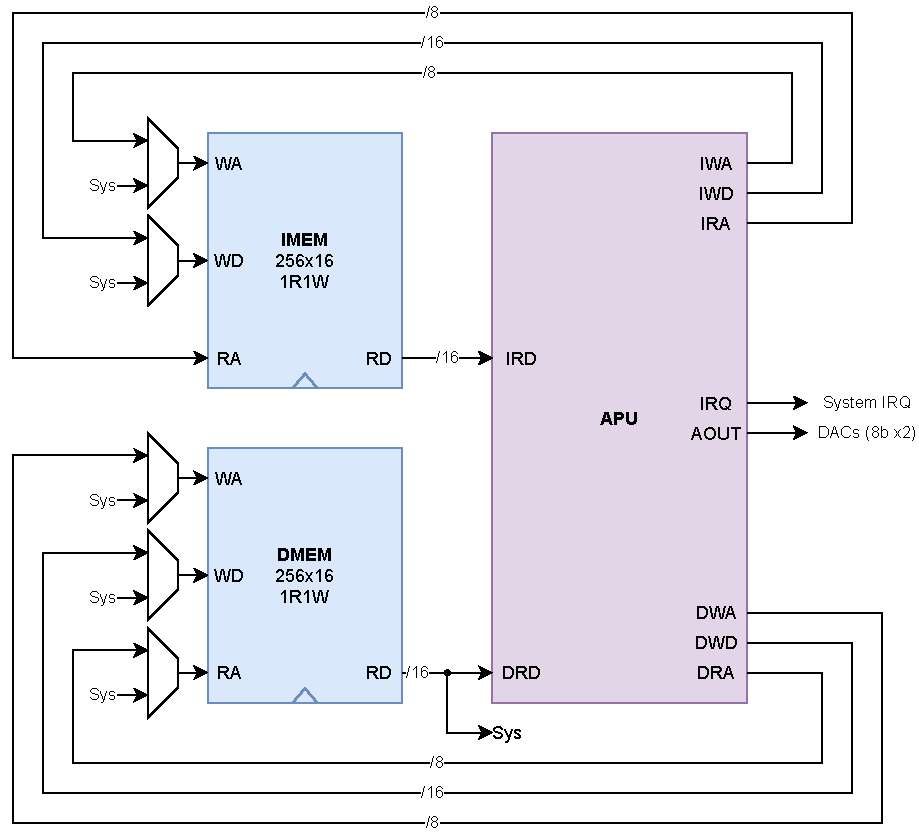
\includegraphics[width=0.6\textwidth]{diagrams/apu_mem_arch.pdf}
\end{figure}


\begin{itemize}
	\item IMEM:
	\begin{itemize}
		\item Contains the APU program instructions. Each instruction is 16 bits in size.
		\item Upper 8 slots contain a copy of the APU's general purpose registers
		\item The system has write-only access when the APU is halted, and no access when the APU is running
	\end{itemize}
	\item DMEM:
	\begin{itemize}
		\item Contains sample ring buffers used for wave tables or for buffering PCM data from the system
		\item Contains program temporary variables that don't fit into registers or need to be indexed
		\item Upper 8 slots contain a copy of the APU's general purpose registers
		\item The system has read-write access at all times, at a lower priority than the APU (system access stalls when the APU is accessing DMEM)
	\end{itemize}
\end{itemize}

8 general-purpose registers are available to APU programs. The register contents are mirrored across IMEM and DMEM, so that two independent register reads can take place simultaneously. Register writeback of one instruction is overlapped with instruction fetch of the next instruction. A typical register-to-register instruction (e.g. an add) executes in two cycles, performs 3 memory reads and 2 memory writes.

\subsubsection*{Arithmetic}

There are two data types used by APU instructions:

\begin{itemize}
	\item 16-bit integers
	\item Packed pairs of 8-bit integers (SIMD)
\end{itemize}

The former is useful for control variables and for phase accumulation of digital oscillators. The latter is used for SIMD processing of stereo sampling pairs. All 8-bit arithmetic is signed-saturating. 16-bit arithmetic can generally be either signed-saturating or normal modular arithmetic.

\subsubsection*{Input/Output}

The APU performs all calculations necessary to produce a 2$\times$8-bit stereo sample pair, then outputs this to the external DACs (probably some kind of sigma delta thing) with an {\tt out} instruction. The APU then stalls until the end of the audio sample period, whereupon it begins calculating the next samples.

For PCM sample streaming, the APU accesses ring buffers in DMEM, in the same way that it access DMEM wavetables for local synthesis. The system tops up the ring buffers by writing to DMEM, triggered by APU interrupts.

The {\tt irq} instruction can generate a system interrupt, which is mainly useful for half-empty or quarter-empty interrupts for PCM ring buffers.

\subsection{Instruction Set}

The two main instruction formats are:

{\bf R format}

\begin{bytefield}[endianness=big]{16}
\bitheader{0,4,5,7,8,10,11,15} \\
\bitbox{5}{{\tt opcode}} \bitbox{3}{{\tt rd}} \bitbox{3}{{\tt rs}} \bitbox{5}{\reservedfield}
\end{bytefield}

{\bf I format}

\begin{bytefield}[endianness=big]{16}
\bitheader{0,7,8,10,11,15} \\
\bitbox{5}{{\tt opcode}} \bitbox{3}{{\tt rd}} \bitbox{8}{{\tt imm}}
\end{bytefield}

\subsection*{Example Programs}

\subsubsection*{Wave channel}

\begin{lstlisting}
.imem                     ; List instruction memory contents
	ld r1, [#freq]        ; Initialise frequency from data memory
	li r0, #0             ; Initialise phase to 0
loop:
	addm16 r0, r1         ; Modular 16-bit addition to advance phase
	ldw r2, [r0, #sine]   ; Look up 2x8-bit samples in sine wave table
	out r2                ; Output samples to DAC, stall until next sample
	b loop                ; Repeat forever

.dmem                     ; List data memory contents
sine:
	...
freq:
	.hword 0x1234
\end{lstlisting}

\subsubsection{Wave channel, controllable frequency}

\begin{lstlisting}
.imem
loop:
	ld r1, [#freq]        ; Fetch frequency stored in memory
	ll r0, [#phase]       ; Fetch phase stored in memory, and set exclusive flag
	addm16 r0, r1         ; Increment phase by frequency
	sc r0, [#phase]       ; Store phase back into memory if still exclusive
	ldw r0, [r0, #sine]   ; Load wave sample from sine table
	out r0                ; Output 2x8-bit samples from r0
	b loop                ; Always jump to loop

.dmem
sine:
	...
freq:
	.hword 0x1234
phase:
	.hword 0
\end{lstlisting} 

\subsubsection{Wave channel, controllable volume with decay}

\begin{lstlisting}
.imem
loop:
	ld r1, [#freq]       ; Atomic update phase based on frequency
	ll r0, [#phase]
	addm16 r0, r1
	sc r0, [#phase]
	ld r2, [#decay]      ; Atomic update volume based on linear decay
	ll r1, [#volume]
	sub16 r1, r2
	sc r1, [#volume]
	ldw r0, [r0, #sine]  ; Look up wave table based on phase
	movhl r1, r1         ; Duplicate upper byte of volume
	mul48 r0, r1         ; Multiply each sample by 4 volume MSBs
	out
	b loop

.dmem
sine:
	...
freq:
	.hword 0x1234
phase:
	.hword 0
decay:
	.hword 0xabcd
volume:
	.hword 0
\end{lstlisting}

\subsubsection{Multiple wave channels}


\section{Bus Fabric and Memory Subsystem}

Bus fabric is digital plumbing. A master, such as a processor, requests a read or write on some address; the bus fabric routes the request to the correct slave device, and routes the response back. RISCBoy implements two bus fabric standards:

\begin{itemize}
\item AMBA 3 AHB-Lite connects masters to high-performance devices such as SRAM controllers
\item AMBA 3 APB connects to simple devices such as a UART
\end{itemize}

Figure \ref{diagram:crossbar_structure} shows the structure of the AHB-Lite crossbar ({\tt ahbl\_crossbar.v}). The crossbar is shown in context in figure \ref{diagram:system_arch}. An independent AHB-Lite datapath connects each of $m$ masters to each of $n$ slaves. One master can address one slave at a time, and one slave can be in data-phase with one master at a time; subject to these constraints, up to $\min(m,n)$ independent transfers can take place in a single machine clock cycle.

Some claim AHB-Lite does not "support" multi-master arbitration. Their problem is a lack of enthusiasm: motorbikes do not "support" wheelies by design, but are excellent at it.

\begin{figure}[!htb]
\centering
\caption{AHB-Lite crossbar, module-level block diagram} \includegraphics[width=0.6\textwidth]{diagrams/crossbar_structure.pdf}
\label{diagram:crossbar_structure}
\end{figure}

Each master is under the illusion that it is the only master in the system, but that slaves sometimes take longer to respond. During this waiting period, the slave may actually have fielded multiple transactions from higher-priority masters; this interaction is handled by the slave's AHB-Lite arbiter, and is transparent to the masters.

One of the crossbar's slave ports is attached to an AHBL-APB bridge. This bridge appears as a slave to the AHB portion of the bus fabric, and as a master to the APB portion. There are three main benefits to this scheme:

\begin{itemize}
	\item APB is fundamentally simpler
	\begin{itemize}
		\item This keeps peripheral gate count down
		\item The peripherals on the APB bus do not need the full AHB-Lite bandwidth anyway
	\end{itemize}
	\item Fewer AHB-Lite slaves
	\begin{itemize}
		\item There is a nonlinear area scaling associated with adding slaves to the AHB-Lite fabric
		\item This would also add extra gate delays to a fairly critical data path
	\end{itemize}
	\item One APB master
	\begin{itemize}
		\item AHB-Lite masters get arbitrated down to one inside the AHB-Lite crossbar. APB slaves do not care who is addressing them.
		\item Different masters accessing different APB slaves will have to queue to use the bridge, even though they could theoretically proceed simultaneously
		\item However, area/complexity vs performance tradeoff is more than worth it for slow peripherals
		\item Multi-master APB is easy to implement, but never used in practice, due to the above tradeoff
	\end{itemize}
\end{itemize}

The splitter and arbiter modules in the AHB-Lite crossbar can also be used on their own. Arbitrary multi-layer busfabric topologies should be possible with these two components.

Currently, the RISCBoy busfabric does not support AHB-Lite bursts (TODO), and the masters do not use them.

\subsection{AHB-Lite Primer}

For a full understanding of the bus standard used by RISCBoy, read through ARM's AMBA 3 AHB-Lite spec. This document is mirrored in the {\tt reference} folder in the GitHub repository, and gives a clear and comprehensive breakdown of AHB-Lite. However, the following overview should provide sufficient understanding of the standard to read through the Verilog.

Transactions take place in two phases, named the address phase and the data phase. During the address phase, the master asserts signals which control the nature of the transfer, such as the address, whether the transfer is a read or write, protection/permission information, the width of the data, and so on. During the data phase, data is asserted on either the read or write data bus ({\tt hrdata} and {\tt hwdata}), but never both. {\tt hrdata} is driven by the slave, and {\tt hwdata} by the master.

The central conceit of AHB-Lite is that these two phases are {\it pipelined}. Whilst the master is asserting or accepting data for an earlier transaction (currently in data phase), it concurrently asserts address and control information for a later transaction (currently in address phase). As is generally the case with pipelining, the goal is to enable higher clock frequencies with undiminished work-per-clock.

\begin{figure}[H]
\centering
\caption{AHB-Lite transfers, a simple example}
\includegraphics[width=0.9\textwidth]{waves/ahbl_basic.pdf}
\label{diagram:ahbl_basic}
\end{figure}

In figure \ref{diagram:ahbl_basic}, a master carries out two AHB-Lite transactions: a write to address A, followed by a read from address B. Only a subset of AHB-Lite signals are shown on the diagram. {\tt htrans}, {\tt haddr}, and {\tt hwrite} are driven by the master, during the address phase; the other two are data phase signals. {\tt htrans} indicates the type of transfer the master next wishes to perform, which is one of {\tt IDLE}, {\tt NSEQ} (non-sequential), {\tt SEQ} and {\tt BUSY}. The latter two are exclusive to burst transactions, which are not used in RISCBoy. (See the ARM spec if you do want details.)

Sometimes a slave is unable to service a request immediately, as shown in figure \ref{diagram:ahbl_basic_stall}. {\tt hready} is a data phase signal, which signifies the end of the current data phase.

\begin{figure}[H]
\centering
\caption{AHB-Lite transfers, simple example with stalling}
\includegraphics[width=0.9\textwidth]{waves/ahbl_basic_stall.pdf}
\label{diagram:ahbl_basic_stall}
\end{figure}

This slave needs two cycles to perform each data phase; perhaps it is an SRAM capable of running only at half the system clock speed. Therefore, {\tt hready} is low for one cycle, and high for the second (last) cycle of each data phase. The master drives {\tt hwdata} for the duration of A's data phase, waiting for the slave to signal completion. {\tt hrdata}, on the other hand, is invalid until the final cycle of a read data phase.

Note that an address phase does not complete until the preceding transfer's data phase completes. In figure \ref{diagram:ahbl_basic_stall}, address B (and associated address-phase signals) continue to be driven until the A data phase completes. {\tt IDLE} transactions do have a data phase, which always completes immediately. Consequently, {\tt hready} idles high while the bus is in an idle state. This is why A's address phase completes immediately in the figure.

In a practical system, there are multiple slaves. Each drives a signal called {\tt hreadyout}, to indicate that {\it that slave} is ready. The bus fabric tracks which slave the master is currently accessing in the data phase, and selects that slave's {\tt hreadyout} to be the global {\tt hready}. To see why this is necessary, think about the situation where a master is in data phase with one slave, and address phase with a different slave.

\subsection{Multi-Master Operation}

In a single-master busfabric, {\tt hready} is a global signal, which causes the entire AHB-Lite state machine (masters, slaves, fabric, the lot) to advance. Where multiple masters are concerned, {\tt hready} is more subtle; in part it is a per-master stall signal. At this point we need to be more specific about the relationship between {\tt hreadyout} and {\tt hready}.

Any AHB-Lite slave port (of which there is one on the master side of the splitter, $n$ on the master side of the arbiter, and one on each slave device) has an output called {\tt hreadyout}, which indicates the slave's readiness. Each of these ports also has an input called {\tt hready}, which indicates that the data phase is ending for the master who is connected to this slave (which does not mean that it is in data phase with {\it this} slave; it may be addressing this slave while in data phase with another). {\tt hready} is a function of {\tt hreadyout}s and bus state. The connections between masters, splitters, arbiters and slaves are shown in figure \ref{diagram:crossbar_structure}.

In the single-layer crossbar on RISCBoy, each system AHB-Lite slave is the slave of an arbiter, which is the slave of several splitters, each of which is the slave of a system master. As a general rule, the busfabric must filter system slaves' {\tt hreadyout}s up to each system master, tie {\tt hreadyout}s across to {\tt hready}s at the very top of the busfabric, and then distribute these {\tt hready} signals down to the correct system slaves.

\subsubsection{Multiple Masters, One Slave}

The arbiters are the most complex busfabric component, so it is instructive to consider interactions between multiple masters and a single slave, which are mediated by one arbiter. There are additional complexities when we combine arbiters and splitters to build a crossbar, which are discussed in the next section.

In figure \ref{diagram:ahbl_mm_simult1}, two masters attempt to access a single slave simultaneously. Assume that master 0 always wins address-phase arbitration:

\begin{figure}[H]
\centering
\caption{AHB-Lite transfers, two masters access one slave}
\includegraphics[width=0.9\textwidth]{waves/ahbl_mm_simult1.pdf}
\label{diagram:ahbl_mm_simult1}
\end{figure}

Again, we assume the slave requires 2 cycles to complete each data phase.

If we look at each master's trace, there is no indication at all that there is more than one master in the system: they present an address, and subsequently the transaction completes. Likewise, the slave neither knows nor cares that there are multiple masters: it simply carries out transactions according to the address-phase signals it sees. All of the smoke, mirrors and machinery are inside of the arbiter.

One odd feature of this trace is that, when the slave sees the address B, no master is asserting this address.

\begin{enumerate}
	\item Initially, both masters assert {\tt IDLE}; {\tt IDLE} data phases complete in one cycle
	\item {\tt IDLE} data phases are concurrent with A, B address phases, so these {\it also} complete immediately
	\item From the master 1's point of view, transaction B proceeds immediately to data phase.
	\item From both the master 0's and the slave's point of view, transaction A proceeds immediately to data phase
	\item Whilst the slave is in data phase for A, it is simultaneously in address phase for B
	\item When A data phase completes, master 0 is signaled, and B proceeds to data phase at the slave
	\item When B data phase completes, master 1 is signaled
\end{enumerate}

More concisely put, the first clock cycle of a given transaction's data phase may differ between the slave and master, but the {\it last} cycle of that data phase is always the same clock cycle. The slave address phase will occur some time between the master address phase starting, and the slave data phase starting. These are strong enough guarantees for correct operation.

Based on this discussion, the AHB-Lite arbiters need the facility to buffer one address-phase request, per master. A buffered request will be applied before any new requests from that master, but after any higher-priority requests. There is a nonzero hardware cost to this buffering, but there are clear engineering benefits to keeping this complexity confined to the arbiters, as they are the only component in the busfabric which is explicitly "multi master".

\begin{figure}[H]
\centering
\caption{AHB-Lite transfers, two masters access one slave, with low-priority back-to-back}
\includegraphics[width=0.9\textwidth]{waves/ahbl_mm_simult2.pdf}
\label{diagram:ahbl_mm_simult2}
\end{figure}

Figure \ref{diagram:ahbl_mm_simult2} shows the same sequence of events as figure \ref{diagram:ahbl_mm_simult1}, except master 1 now performs two back-to-back transactions. Once B's slave address phase completes, the arbiter's request buffer is cleared, and the C request passes transparently through the arbiter to the slave. Again, the only indication to master 1 of any master 0 activity is increased latency.

There is a different case which requires the arbiter's request buffer, shown in figure \ref{diagram:ahbl_mm_simult3}.

\begin{figure}[H]
\centering
\caption{AHB-Lite arbiter: simultaneous request buffer writes}
\includegraphics[width=0.9\textwidth]{waves/ahbl_mm_simult3.pdf}
\label{diagram:ahbl_mm_simult3}
\end{figure}

At the instant where D address phase is asserted, {\tt hready0} is high, because master 0 previously asserted an {\tt IDLE} transfer. However, the slave is not ready. In this case, the arbiter needs to buffer master 0's request, even though it is the highest-priority master. The buffered request is cleared once its slave address phase completes, as usual.

On the next cycle, B's data phase completes, and master 1 also considers this to be the end of the C address phase. The arbiter must write the C request into master 1's request buffer. Master 0's buffered request will continue to take priority over master 1's buffered request, until the first buffer is cleared.

There is one final case, for two masters accessing one slave, which is worth being aware of (figure \ref{diagram:ahbl_mm_latearrival}).

\begin{figure}[H]
\centering
\caption{AHB-Lite arbiter: late arrival of high priority request}
\includegraphics[width=0.9\textwidth]{waves/ahbl_mm_latearrival.pdf}
\label{diagram:ahbl_mm_latearrival}
\end{figure}

Whilst {\tt hreadyout} is low, the C address briefly appears on the slave bus, before being replaced by the higher-priority D request. \textbf{This is a departure from the AHB-Lite standard}, which stipulates the address must be constant during this time. This is deliberate, and easily amended. Slaves are generally insensitive to address-phase request during this time (as there is no performance benefit to latching APR before {\tt hreadyout}, due to the way the bus operates), and this avoids a priority inversion, reducing average latency for higher-priority masters. If you find something that this breaks, write me an angry email! I would be interested to see such a slave.

The D request causes the low-priority C request to be buffered; the B data phase completes on this cycle, hence, from master 0's point of view, the C address phase does too.

\subsubsection{Full Crossbar}

The previous section discussed some cases where multiple masters access a single slave, and showed how the arbiter safely navigates them. There are yet more issues to consider when multiple masters and multiple slaves are involved, which must be handled without added latency cycles, and with minimal extra gate delay.

For example, a master may be engaged in address phase with one arbiter and data phase with another arbiter simultaneously, via a splitter, and these two arbiters will not necessarily signal {\tt hreadyout} at the same time. Consequently, a master may have a positive {\tt hready}, filtered from its data phase arbiter, when its address phase arbiter has a negative {\tt hreadyout}, which requires action on the arbiter's part.

There is also the issue that being in data phase with an arbiter does not mean you are genuinely in data phase with the arbitrated slave; in fact, a very simple sequence of events (all masters {\tt IDLE} $\to$ all masters {\tt NSEQ}) will put all masters simultaneously in data phase with the same arbiter. The arbiter behaviour described in the previous section should allow us to abstract this away, provided we can deal with the first issue safely.

Splitters will filter their slaves' {\tt hreadyout}s based on which is currently in data phase, and present it on their own slave port. Arbiters will present their slave's {\tt hreadyout} on any master-facing ports which are in data phase with the arbiter, and will present ${\tt hreadyout} = 1$ on any idle ports.

Splitters will fan their {\tt hready} signal out to all of their slaves; a low {\tt hready} directed at a slave you are not engaged with is harmless.

\subsection{Memories}

RISCBoy possesses two memory areas for data and code: an external SRAM (512 kiB, 16 b wide, asynchronous), and internal RAM (8 kiB, 32 b wide, synchronous), assembled from FPGA block RAMs. The former is the main system memory, which most games will simply load into as a flat image; the latter is intended to be used for processor stack, and some critical code sections, including ISRs. Internal RAM also contains the first-stage bootloader, as it can be initialised during FPGA configuration, so is a convenient place to put the first few thousand instructions the processor will execute at start-of-day. SRAM was chosen for the external memory due to the low initial access latency -- this permits reasonable performance without building complex cache hierarchies into the system bus masters. On a larger FPGA we could consider something like HyperRAM, or even DDRx SDRAM.

Both memories need to be interfaced to the AHB-lite system bus. SRAMs aren't too complex, but they can be a little fiddly to use efficiently due to the timing of AHB-lite -- in particular, the alignment of {\tt haddr} and {\tt hwdata} is more or less the opposite of what you want for a synchronous SRAM.

The internal SRAM can perform one 32-bit read or write per cycle. The external SRAM can also service a 32-bit AHB-lite read every cycle, because it is double-pumped; the controller performs two back-to-back 16 bit SRAM reads in one clock cycle. However, writes to external SRAM are limited to 16 bits per clock cycle, due to the timing of the {\tt WE} pin, which is deasserted part way through each access. This is reasonable -- reads are more common than writes, for almost any workload. However, special cases like the processor stack will benefit from the improved write performance of IRAM.

\subsubsection{Internal RAM}

Synchronous single-port SRAMs typically behave as follows:

\begin{itemize}
	\item Address, write data and write enable are presented on one clock
	\item Read data is available on the next clock (and the whole process is pipelined)
	\item Byte-enables allow narrow writes to be performed without a read-modify-write sequence.
\end{itemize}

This is shown in figure \ref{diagram:sync_sram_only}. However, in AHB-lite, read and write data are both presented during the data phase, which begins on the cycle after the address phase completes. The timing of this is shown in figure \ref{diagram:sync_sram_ahb_access}. Note the difference in timing between {\tt wdata} in figure \ref{diagram:sync_sram_only} and {\tt hwdata} in figure \ref{diagram:sync_sram_ahb_access}.


\begin{figure}[H]
\centering
\caption{Timing of synchronous SRAM interface}
\includegraphics[width=0.7\textwidth]{waves/sync_sram_only.pdf}
\label{diagram:sync_sram_only}
\end{figure}


\begin{figure}[H]
\centering
\caption{Timing of AHB-lite SRAM accesses, showing write data misalignment}
\includegraphics[width=0.7\textwidth]{waves/sync_sram_ahb_access.pdf}
\label{diagram:sync_sram_ahb_access}
\end{figure}

The issue is that, as we can't source signals from the future, the SRAM write cycle must be delayed so that write address is aligned with write data. However, if the next transfer is a read, there is a collision: the delayed write address would need to be presented on the same cycle as the read address, which is impossible for a single-port SRAM. One way to resolve this is to simply insert wait states on write access, shown in figure \ref{diagram:sync_sram_ahb_stall}.

\begin{figure}[H]
\centering
\caption{AHB-lite SRAM access: resolving address collision with wait states}
\includegraphics[width=0.8\textwidth]{waves/sync_sram_ahb_stall.pdf}
\label{diagram:sync_sram_ahb_stall}
\end{figure}

This works, but the performance cost is significant if you are constantly swapping back and forth between reads and writes (like, say, a processor!). This needn't be so. Noting that:

\begin{itemize}
	\item Multiple consecutive writes are fine; all addresses are delayed equally, so do not collide
	\item Write-to-read has a single collision, and no more
	\item A run of consecutive reads is always followed by either an idle cycle or a write cycle (by definition)
	\item Read-to-write leaves the SRAM idle for one cycle; this is seen in figure \ref{diagram:sync_sram_ahb_stall}
\end{itemize}

If we are able to buffer a single write, and hold onto it until the SRAM is idle (either AHB idle or read-to-write), we never need wait states. The only additional wrinkle is that, if a read is issued to an address we are currently holding a buffered write to, we will need to merge the buffered write data into the read data on-the-fly. As the write may be narrower than the SRAM, this needs to be done on a byte-by-byte basis. Use of a write buffer is shown in figure \ref{diagram:sync_sram_ahb_buffer}.

\begin{figure}[H]
\centering
\caption{AHB-lite SRAM access: resolving address collision with a write buffer}
\includegraphics[width=0.75\textwidth]{waves/sync_sram_ahb_buffer.pdf}
\label{diagram:sync_sram_ahb_buffer}
\end{figure}

It's probably worth staring at for a short while. Key observations for figure \ref{diagram:sync_sram_ahb_buffer}:

\begin{itemize}
	\item SRAM reads are always aligned with AHB-lite reads, to avoid adding latency
	\item SRAM writes are in-order with respect to other SRAM writes (otherwise we'd need more buffering)
	\item An SRAM write can be deferred for any number of read cycles, after which the SRAM address bus will be free
	\item The data buffer is only needed for write-to-read, not write-to-write or write-to-idle.
\end{itemize}


\subsubsection{Main Memory}

Main memory consists of a 16-bit-wide, 512 kiB asynchronous SRAM. The rough timing of read and write cycles is shown below (just signal alignment, no timing parameters):

(TODO)

Currently the controller requires a single cycle for each 16-bit access, and services 32-bit accesses from the busfabric as two back-to-back external access cycles; a single wait state is inserted via {\tt hready}. At RISCBoy's target clock frequency of 36 MHz, this cuts the available bandwidth down to 72 MiB/s.

The part used has a 10 ns access time, and RISCBoy is targeting around a 36 MHz system clock period (\textasciitilde 28 ns), so with some care we may be able to perform two reads in the same clock cycle, using a DDR output on the least-significant address bit, and an optional negedge capture fed into the lower half of the AHB-lite data bus. This means we can service one 32-bit AHB-lite read each cycle, which is ideal for a 32-bit processor with up to 32-bit instructions!

Writes are more problematic: due to the timing of the {\tt WE} pin, we need a full cycle for each 16-bit write cycle, so 32-bit writes will stall for one cycle. Write-intensive memory regions such as the processor stack should be located in IRAM if possible, to avoid this performance penalty.



\end{document}
